% Created by tikzDevice version 0.10.1 on 2016-11-20 12:15:34
% !TEX encoding = UTF-8 Unicode
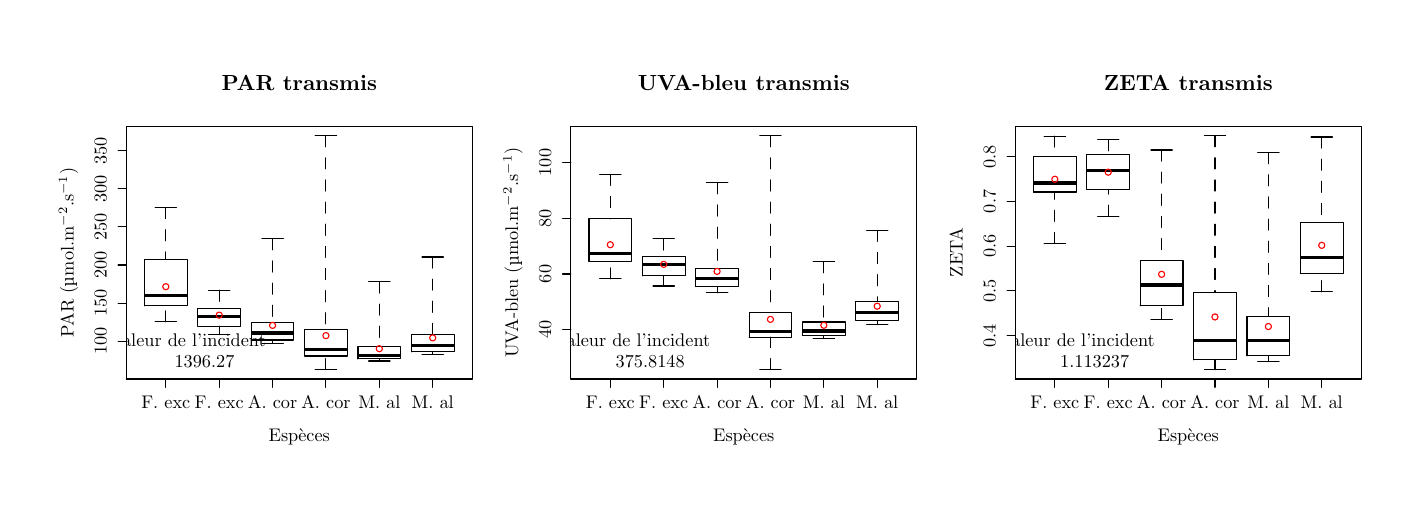
\begin{tikzpicture}[x=1pt,y=1pt, scale=0.75]
\definecolor{fillColor}{RGB}{255,255,255}
\path[use as bounding box,fill=fillColor,fill opacity=0.00] (0,0) rectangle (650.43,216.81);
\begin{scope}
\path[clip] ( 47.52, 47.52) rectangle (214.17,169.29);
\definecolor{drawColor}{RGB}{0,0,0}

\path[draw=drawColor,line width= 1.2pt,line join=round] ( 56.26, 87.71) -- ( 76.84, 87.71);

\path[draw=drawColor,line width= 0.4pt,dash pattern=on 4pt off 4pt ,line join=round,line cap=round] ( 66.55, 75.05) -- ( 66.55, 82.82);

\path[draw=drawColor,line width= 0.4pt,dash pattern=on 4pt off 4pt ,line join=round,line cap=round] ( 66.55,130.12) -- ( 66.55,105.25);

\path[draw=drawColor,line width= 0.4pt,line join=round,line cap=round] ( 61.41, 75.05) -- ( 71.69, 75.05);

\path[draw=drawColor,line width= 0.4pt,line join=round,line cap=round] ( 61.41,130.12) -- ( 71.69,130.12);

\path[draw=drawColor,line width= 0.4pt,line join=round,line cap=round] ( 56.26, 82.82) --
	( 76.84, 82.82) --
	( 76.84,105.25) --
	( 56.26,105.25) --
	( 56.26, 82.82);

\path[draw=drawColor,line width= 1.2pt,line join=round] ( 81.98, 77.50) -- (102.56, 77.50);

\path[draw=drawColor,line width= 0.4pt,dash pattern=on 4pt off 4pt ,line join=round,line cap=round] ( 92.27, 68.94) -- ( 92.27, 72.98);

\path[draw=drawColor,line width= 0.4pt,dash pattern=on 4pt off 4pt ,line join=round,line cap=round] ( 92.27, 90.30) -- ( 92.27, 81.58);

\path[draw=drawColor,line width= 0.4pt,line join=round,line cap=round] ( 87.13, 68.94) -- ( 97.41, 68.94);

\path[draw=drawColor,line width= 0.4pt,line join=round,line cap=round] ( 87.13, 90.30) -- ( 97.41, 90.30);

\path[draw=drawColor,line width= 0.4pt,line join=round,line cap=round] ( 81.98, 72.98) --
	(102.56, 72.98) --
	(102.56, 81.58) --
	( 81.98, 81.58) --
	( 81.98, 72.98);

\path[draw=drawColor,line width= 1.2pt,line join=round] (107.70, 69.72) -- (128.27, 69.72);

\path[draw=drawColor,line width= 0.4pt,dash pattern=on 4pt off 4pt ,line join=round,line cap=round] (117.99, 64.55) -- (117.99, 66.31);

\path[draw=drawColor,line width= 0.4pt,dash pattern=on 4pt off 4pt ,line join=round,line cap=round] (117.99,115.06) -- (117.99, 74.88);

\path[draw=drawColor,line width= 0.4pt,line join=round,line cap=round] (112.84, 64.55) -- (123.13, 64.55);

\path[draw=drawColor,line width= 0.4pt,line join=round,line cap=round] (112.84,115.06) -- (123.13,115.06);

\path[draw=drawColor,line width= 0.4pt,line join=round,line cap=round] (107.70, 66.31) --
	(128.27, 66.31) --
	(128.27, 74.88) --
	(107.70, 74.88) --
	(107.70, 66.31);

\path[draw=drawColor,line width= 1.2pt,line join=round] (133.42, 61.59) -- (153.99, 61.59);

\path[draw=drawColor,line width= 0.4pt,dash pattern=on 4pt off 4pt ,line join=round,line cap=round] (143.70, 52.03) -- (143.70, 58.63);

\path[draw=drawColor,line width= 0.4pt,dash pattern=on 4pt off 4pt ,line join=round,line cap=round] (143.70,164.78) -- (143.70, 71.39);

\path[draw=drawColor,line width= 0.4pt,line join=round,line cap=round] (138.56, 52.03) -- (148.85, 52.03);

\path[draw=drawColor,line width= 0.4pt,line join=round,line cap=round] (138.56,164.78) -- (148.85,164.78);

\path[draw=drawColor,line width= 0.4pt,line join=round,line cap=round] (133.42, 58.63) --
	(153.99, 58.63) --
	(153.99, 71.39) --
	(133.42, 71.39) --
	(133.42, 58.63);

\path[draw=drawColor,line width= 1.2pt,line join=round] (159.13, 58.92) -- (179.71, 58.92);

\path[draw=drawColor,line width= 0.4pt,dash pattern=on 4pt off 4pt ,line join=round,line cap=round] (169.42, 56.20) -- (169.42, 57.24);

\path[draw=drawColor,line width= 0.4pt,dash pattern=on 4pt off 4pt ,line join=round,line cap=round] (169.42, 94.30) -- (169.42, 63.31);

\path[draw=drawColor,line width= 0.4pt,line join=round,line cap=round] (164.28, 56.20) -- (174.56, 56.20);

\path[draw=drawColor,line width= 0.4pt,line join=round,line cap=round] (164.28, 94.30) -- (174.56, 94.30);

\path[draw=drawColor,line width= 0.4pt,line join=round,line cap=round] (159.13, 57.24) --
	(179.71, 57.24) --
	(179.71, 63.31) --
	(159.13, 63.31) --
	(159.13, 57.24);

\path[draw=drawColor,line width= 1.2pt,line join=round] (184.85, 63.70) -- (205.43, 63.70);

\path[draw=drawColor,line width= 0.4pt,dash pattern=on 4pt off 4pt ,line join=round,line cap=round] (195.14, 59.55) -- (195.14, 60.65);

\path[draw=drawColor,line width= 0.4pt,dash pattern=on 4pt off 4pt ,line join=round,line cap=round] (195.14,106.33) -- (195.14, 68.98);

\path[draw=drawColor,line width= 0.4pt,line join=round,line cap=round] (190.00, 59.55) -- (200.28, 59.55);

\path[draw=drawColor,line width= 0.4pt,line join=round,line cap=round] (190.00,106.33) -- (200.28,106.33);

\path[draw=drawColor,line width= 0.4pt,line join=round,line cap=round] (184.85, 60.65) --
	(205.43, 60.65) --
	(205.43, 68.98) --
	(184.85, 68.98) --
	(184.85, 60.65);
\end{scope}
\begin{scope}
\path[clip] (  0.00,  0.00) rectangle (650.43,216.81);
\definecolor{drawColor}{RGB}{0,0,0}

\path[draw=drawColor,line width= 0.4pt,line join=round,line cap=round] ( 66.55, 47.52) -- (195.14, 47.52);

\path[draw=drawColor,line width= 0.4pt,line join=round,line cap=round] ( 66.55, 47.52) -- ( 66.55, 43.56);

\path[draw=drawColor,line width= 0.4pt,line join=round,line cap=round] ( 92.27, 47.52) -- ( 92.27, 43.56);

\path[draw=drawColor,line width= 0.4pt,line join=round,line cap=round] (117.99, 47.52) -- (117.99, 43.56);

\path[draw=drawColor,line width= 0.4pt,line join=round,line cap=round] (143.70, 47.52) -- (143.70, 43.56);

\path[draw=drawColor,line width= 0.4pt,line join=round,line cap=round] (169.42, 47.52) -- (169.42, 43.56);

\path[draw=drawColor,line width= 0.4pt,line join=round,line cap=round] (195.14, 47.52) -- (195.14, 43.56);

\node[text=drawColor,anchor=base,inner sep=0pt, outer sep=0pt, scale=  0.66] at ( 66.55, 33.26) {F. exc};

\node[text=drawColor,anchor=base,inner sep=0pt, outer sep=0pt, scale=  0.66] at ( 92.27, 33.26) {F. exc};

\node[text=drawColor,anchor=base,inner sep=0pt, outer sep=0pt, scale=  0.66] at (117.99, 33.26) {A. cor};

\node[text=drawColor,anchor=base,inner sep=0pt, outer sep=0pt, scale=  0.66] at (143.70, 33.26) {A. cor};

\node[text=drawColor,anchor=base,inner sep=0pt, outer sep=0pt, scale=  0.66] at (169.42, 33.26) {M. al};

\node[text=drawColor,anchor=base,inner sep=0pt, outer sep=0pt, scale=  0.66] at (195.14, 33.26) {M. al};

\path[draw=drawColor,line width= 0.4pt,line join=round,line cap=round] ( 47.52, 65.76) -- ( 47.52,157.55);

\path[draw=drawColor,line width= 0.4pt,line join=round,line cap=round] ( 47.52, 65.76) -- ( 43.56, 65.76);

\path[draw=drawColor,line width= 0.4pt,line join=round,line cap=round] ( 47.52, 84.11) -- ( 43.56, 84.11);

\path[draw=drawColor,line width= 0.4pt,line join=round,line cap=round] ( 47.52,102.47) -- ( 43.56,102.47);

\path[draw=drawColor,line width= 0.4pt,line join=round,line cap=round] ( 47.52,120.83) -- ( 43.56,120.83);

\path[draw=drawColor,line width= 0.4pt,line join=round,line cap=round] ( 47.52,139.19) -- ( 43.56,139.19);

\path[draw=drawColor,line width= 0.4pt,line join=round,line cap=round] ( 47.52,157.55) -- ( 43.56,157.55);

\node[text=drawColor,rotate= 90.00,anchor=base,inner sep=0pt, outer sep=0pt, scale=  0.66] at ( 38.02, 65.76) {100};

\node[text=drawColor,rotate= 90.00,anchor=base,inner sep=0pt, outer sep=0pt, scale=  0.66] at ( 38.02, 84.11) {150};

\node[text=drawColor,rotate= 90.00,anchor=base,inner sep=0pt, outer sep=0pt, scale=  0.66] at ( 38.02,102.47) {200};

\node[text=drawColor,rotate= 90.00,anchor=base,inner sep=0pt, outer sep=0pt, scale=  0.66] at ( 38.02,120.83) {250};

\node[text=drawColor,rotate= 90.00,anchor=base,inner sep=0pt, outer sep=0pt, scale=  0.66] at ( 38.02,139.19) {300};

\node[text=drawColor,rotate= 90.00,anchor=base,inner sep=0pt, outer sep=0pt, scale=  0.66] at ( 38.02,157.55) {350};
\end{scope}
\begin{scope}
\path[clip] (  7.92,  7.92) rectangle (222.09,208.89);
\definecolor{drawColor}{RGB}{0,0,0}

\node[text=drawColor,anchor=base,inner sep=0pt, outer sep=0pt, scale=  0.79] at (130.84,186.32) {\bfseries PAR transmis};

\node[text=drawColor,anchor=base,inner sep=0pt, outer sep=0pt, scale=  0.66] at (130.84, 17.42) {Espèces};

\node[text=drawColor,rotate= 90.00,anchor=base,inner sep=0pt, outer sep=0pt, scale=  0.66] at ( 22.18,108.41) {PAR (µmol.m$^{-2}$.s$^{-1}$)};
\end{scope}
\begin{scope}
\path[clip] (  0.00,  0.00) rectangle (650.43,216.81);
\definecolor{drawColor}{RGB}{0,0,0}

\path[draw=drawColor,line width= 0.4pt,line join=round,line cap=round] ( 47.52, 47.52) --
	(214.17, 47.52) --
	(214.17,169.29) --
	( 47.52,169.29) --
	( 47.52, 47.52);
\end{scope}
\begin{scope}
\path[clip] ( 47.52, 47.52) rectangle (214.17,169.29);
\definecolor{drawColor}{RGB}{0,0,0}

\node[text=drawColor,anchor=base,inner sep=0pt, outer sep=0pt, scale=  0.66] at ( 77.16, 63.36) {Valeur de l'incident};

\node[text=drawColor,anchor=base west,inner sep=0pt, outer sep=0pt, scale=  0.66] at ( 70.79, 53.17) {1396.27};
\definecolor{drawColor}{RGB}{255,0,0}

\path[draw=drawColor,line width= 0.4pt,line join=round,line cap=round] ( 66.55, 92.02) circle (  1.49);

\path[draw=drawColor,line width= 0.4pt,line join=round,line cap=round] ( 92.27, 78.30) circle (  1.49);

\path[draw=drawColor,line width= 0.4pt,line join=round,line cap=round] (117.99, 73.37) circle (  1.49);

\path[draw=drawColor,line width= 0.4pt,line join=round,line cap=round] (143.70, 68.44) circle (  1.49);

\path[draw=drawColor,line width= 0.4pt,line join=round,line cap=round] (169.42, 62.15) circle (  1.49);

\path[draw=drawColor,line width= 0.4pt,line join=round,line cap=round] (195.14, 67.36) circle (  1.49);
\end{scope}
\begin{scope}
\path[clip] (261.69, 47.52) rectangle (428.34,169.29);
\definecolor{drawColor}{RGB}{0,0,0}

\path[draw=drawColor,line width= 1.2pt,line join=round] (270.43,108.15) -- (291.01,108.15);

\path[draw=drawColor,line width= 0.4pt,dash pattern=on 4pt off 4pt ,line join=round,line cap=round] (280.72, 95.78) -- (280.72,104.17);

\path[draw=drawColor,line width= 0.4pt,dash pattern=on 4pt off 4pt ,line join=round,line cap=round] (280.72,146.16) -- (280.72,124.66);

\path[draw=drawColor,line width= 0.4pt,line join=round,line cap=round] (275.58, 95.78) -- (285.86, 95.78);

\path[draw=drawColor,line width= 0.4pt,line join=round,line cap=round] (275.58,146.16) -- (285.86,146.16);

\path[draw=drawColor,line width= 0.4pt,line join=round,line cap=round] (270.43,104.17) --
	(291.01,104.17) --
	(291.01,124.66) --
	(270.43,124.66) --
	(270.43,104.17);

\path[draw=drawColor,line width= 1.2pt,line join=round] (296.15,102.63) -- (316.73,102.63);

\path[draw=drawColor,line width= 0.4pt,dash pattern=on 4pt off 4pt ,line join=round,line cap=round] (306.44, 92.37) -- (306.44, 97.26);

\path[draw=drawColor,line width= 0.4pt,dash pattern=on 4pt off 4pt ,line join=round,line cap=round] (306.44,115.02) -- (306.44,106.69);

\path[draw=drawColor,line width= 0.4pt,line join=round,line cap=round] (301.30, 92.37) -- (311.58, 92.37);

\path[draw=drawColor,line width= 0.4pt,line join=round,line cap=round] (301.30,115.02) -- (311.58,115.02);

\path[draw=drawColor,line width= 0.4pt,line join=round,line cap=round] (296.15, 97.26) --
	(316.73, 97.26) --
	(316.73,106.69) --
	(296.15,106.69) --
	(296.15, 97.26);

\path[draw=drawColor,line width= 1.2pt,line join=round] (321.87, 95.89) -- (342.44, 95.89);

\path[draw=drawColor,line width= 0.4pt,dash pattern=on 4pt off 4pt ,line join=round,line cap=round] (332.16, 89.06) -- (332.16, 92.03);

\path[draw=drawColor,line width= 0.4pt,dash pattern=on 4pt off 4pt ,line join=round,line cap=round] (332.16,142.03) -- (332.16,100.88);

\path[draw=drawColor,line width= 0.4pt,line join=round,line cap=round] (327.01, 89.06) -- (337.30, 89.06);

\path[draw=drawColor,line width= 0.4pt,line join=round,line cap=round] (327.01,142.03) -- (337.30,142.03);

\path[draw=drawColor,line width= 0.4pt,line join=round,line cap=round] (321.87, 92.03) --
	(342.44, 92.03) --
	(342.44,100.88) --
	(321.87,100.88) --
	(321.87, 92.03);

\path[draw=drawColor,line width= 1.2pt,line join=round] (347.59, 70.51) -- (368.16, 70.51);

\path[draw=drawColor,line width= 0.4pt,dash pattern=on 4pt off 4pt ,line join=round,line cap=round] (357.87, 52.03) -- (357.87, 67.69);

\path[draw=drawColor,line width= 0.4pt,dash pattern=on 4pt off 4pt ,line join=round,line cap=round] (357.87,164.78) -- (357.87, 79.52);

\path[draw=drawColor,line width= 0.4pt,line join=round,line cap=round] (352.73, 52.03) -- (363.02, 52.03);

\path[draw=drawColor,line width= 0.4pt,line join=round,line cap=round] (352.73,164.78) -- (363.02,164.78);

\path[draw=drawColor,line width= 0.4pt,line join=round,line cap=round] (347.59, 67.69) --
	(368.16, 67.69) --
	(368.16, 79.52) --
	(347.59, 79.52) --
	(347.59, 67.69);

\path[draw=drawColor,line width= 1.2pt,line join=round] (373.30, 70.68) -- (393.88, 70.68);

\path[draw=drawColor,line width= 0.4pt,dash pattern=on 4pt off 4pt ,line join=round,line cap=round] (383.59, 67.00) -- (383.59, 68.52);

\path[draw=drawColor,line width= 0.4pt,dash pattern=on 4pt off 4pt ,line join=round,line cap=round] (383.59,104.07) -- (383.59, 74.99);

\path[draw=drawColor,line width= 0.4pt,line join=round,line cap=round] (378.45, 67.00) -- (388.73, 67.00);

\path[draw=drawColor,line width= 0.4pt,line join=round,line cap=round] (378.45,104.07) -- (388.73,104.07);

\path[draw=drawColor,line width= 0.4pt,line join=round,line cap=round] (373.30, 68.52) --
	(393.88, 68.52) --
	(393.88, 74.99) --
	(373.30, 74.99) --
	(373.30, 68.52);

\path[draw=drawColor,line width= 1.2pt,line join=round] (399.02, 79.51) -- (419.60, 79.51);

\path[draw=drawColor,line width= 0.4pt,dash pattern=on 4pt off 4pt ,line join=round,line cap=round] (409.31, 73.93) -- (409.31, 75.78);

\path[draw=drawColor,line width= 0.4pt,dash pattern=on 4pt off 4pt ,line join=round,line cap=round] (409.31,119.15) -- (409.31, 85.08);

\path[draw=drawColor,line width= 0.4pt,line join=round,line cap=round] (404.17, 73.93) -- (414.45, 73.93);

\path[draw=drawColor,line width= 0.4pt,line join=round,line cap=round] (404.17,119.15) -- (414.45,119.15);

\path[draw=drawColor,line width= 0.4pt,line join=round,line cap=round] (399.02, 75.78) --
	(419.60, 75.78) --
	(419.60, 85.08) --
	(399.02, 85.08) --
	(399.02, 75.78);
\end{scope}
\begin{scope}
\path[clip] (  0.00,  0.00) rectangle (650.43,216.81);
\definecolor{drawColor}{RGB}{0,0,0}

\path[draw=drawColor,line width= 0.4pt,line join=round,line cap=round] (280.72, 47.52) -- (409.31, 47.52);

\path[draw=drawColor,line width= 0.4pt,line join=round,line cap=round] (280.72, 47.52) -- (280.72, 43.56);

\path[draw=drawColor,line width= 0.4pt,line join=round,line cap=round] (306.44, 47.52) -- (306.44, 43.56);

\path[draw=drawColor,line width= 0.4pt,line join=round,line cap=round] (332.16, 47.52) -- (332.16, 43.56);

\path[draw=drawColor,line width= 0.4pt,line join=round,line cap=round] (357.87, 47.52) -- (357.87, 43.56);

\path[draw=drawColor,line width= 0.4pt,line join=round,line cap=round] (383.59, 47.52) -- (383.59, 43.56);

\path[draw=drawColor,line width= 0.4pt,line join=round,line cap=round] (409.31, 47.52) -- (409.31, 43.56);

\node[text=drawColor,anchor=base,inner sep=0pt, outer sep=0pt, scale=  0.66] at (280.72, 33.26) {F. exc};

\node[text=drawColor,anchor=base,inner sep=0pt, outer sep=0pt, scale=  0.66] at (306.44, 33.26) {F. exc};

\node[text=drawColor,anchor=base,inner sep=0pt, outer sep=0pt, scale=  0.66] at (332.16, 33.26) {A. cor};

\node[text=drawColor,anchor=base,inner sep=0pt, outer sep=0pt, scale=  0.66] at (357.87, 33.26) {A. cor};

\node[text=drawColor,anchor=base,inner sep=0pt, outer sep=0pt, scale=  0.66] at (383.59, 33.26) {M. al};

\node[text=drawColor,anchor=base,inner sep=0pt, outer sep=0pt, scale=  0.66] at (409.31, 33.26) {M. al};

\path[draw=drawColor,line width= 0.4pt,line join=round,line cap=round] (261.69, 71.29) -- (261.69,151.86);

\path[draw=drawColor,line width= 0.4pt,line join=round,line cap=round] (261.69, 71.29) -- (257.73, 71.29);

\path[draw=drawColor,line width= 0.4pt,line join=round,line cap=round] (261.69, 98.14) -- (257.73, 98.14);

\path[draw=drawColor,line width= 0.4pt,line join=round,line cap=round] (261.69,125.00) -- (257.73,125.00);

\path[draw=drawColor,line width= 0.4pt,line join=round,line cap=round] (261.69,151.86) -- (257.73,151.86);

\node[text=drawColor,rotate= 90.00,anchor=base,inner sep=0pt, outer sep=0pt, scale=  0.66] at (252.19, 71.29) {40};

\node[text=drawColor,rotate= 90.00,anchor=base,inner sep=0pt, outer sep=0pt, scale=  0.66] at (252.19, 98.14) {60};

\node[text=drawColor,rotate= 90.00,anchor=base,inner sep=0pt, outer sep=0pt, scale=  0.66] at (252.19,125.00) {80};

\node[text=drawColor,rotate= 90.00,anchor=base,inner sep=0pt, outer sep=0pt, scale=  0.66] at (252.19,151.86) {100};
\end{scope}
\begin{scope}
\path[clip] (222.09,  7.92) rectangle (436.26,208.89);
\definecolor{drawColor}{RGB}{0,0,0}

\node[text=drawColor,anchor=base,inner sep=0pt, outer sep=0pt, scale=  0.79] at (345.01,186.32) {\bfseries UVA-bleu transmis};

\node[text=drawColor,anchor=base,inner sep=0pt, outer sep=0pt, scale=  0.66] at (345.01, 17.42) {Espèces};

\node[text=drawColor,rotate= 90.00,anchor=base,inner sep=0pt, outer sep=0pt, scale=  0.66] at (236.35,108.41) {UVA-bleu (µmol.m$^{-2}$.s$^{-1}$)};
\end{scope}
\begin{scope}
\path[clip] (  0.00,  0.00) rectangle (650.43,216.81);
\definecolor{drawColor}{RGB}{0,0,0}

\path[draw=drawColor,line width= 0.4pt,line join=round,line cap=round] (261.69, 47.52) --
	(428.34, 47.52) --
	(428.34,169.29) --
	(261.69,169.29) --
	(261.69, 47.52);
\end{scope}
\begin{scope}
\path[clip] (261.69, 47.52) rectangle (428.34,169.29);
\definecolor{drawColor}{RGB}{0,0,0}

\node[text=drawColor,anchor=base,inner sep=0pt, outer sep=0pt, scale=  0.66] at (291.33, 63.36) {Valeur de l'incident};

\node[text=drawColor,anchor=base west,inner sep=0pt, outer sep=0pt, scale=  0.66] at (283.31, 53.17) {375.8148};
\definecolor{drawColor}{RGB}{255,0,0}

\path[draw=drawColor,line width= 0.4pt,line join=round,line cap=round] (280.72,112.23) circle (  1.49);

\path[draw=drawColor,line width= 0.4pt,line join=round,line cap=round] (306.44,102.77) circle (  1.49);

\path[draw=drawColor,line width= 0.4pt,line join=round,line cap=round] (332.16, 99.40) circle (  1.49);

\path[draw=drawColor,line width= 0.4pt,line join=round,line cap=round] (357.87, 76.27) circle (  1.49);

\path[draw=drawColor,line width= 0.4pt,line join=round,line cap=round] (383.59, 73.42) circle (  1.49);

\path[draw=drawColor,line width= 0.4pt,line join=round,line cap=round] (409.31, 82.62) circle (  1.49);
\end{scope}
\begin{scope}
\path[clip] (475.86, 47.52) rectangle (642.51,169.29);
\definecolor{drawColor}{RGB}{0,0,0}

\path[draw=drawColor,line width= 1.2pt,line join=round] (484.60,141.93) -- (505.18,141.93);

\path[draw=drawColor,line width= 0.4pt,dash pattern=on 4pt off 4pt ,line join=round,line cap=round] (494.89,112.82) -- (494.89,137.62);

\path[draw=drawColor,line width= 0.4pt,dash pattern=on 4pt off 4pt ,line join=round,line cap=round] (494.89,164.56) -- (494.89,154.86);

\path[draw=drawColor,line width= 0.4pt,line join=round,line cap=round] (489.75,112.82) -- (500.03,112.82);

\path[draw=drawColor,line width= 0.4pt,line join=round,line cap=round] (489.75,164.56) -- (500.03,164.56);

\path[draw=drawColor,line width= 0.4pt,line join=round,line cap=round] (484.60,137.62) --
	(505.18,137.62) --
	(505.18,154.86) --
	(484.60,154.86) --
	(484.60,137.62);

\path[draw=drawColor,line width= 1.2pt,line join=round] (510.32,148.07) -- (530.90,148.07);

\path[draw=drawColor,line width= 0.4pt,dash pattern=on 4pt off 4pt ,line join=round,line cap=round] (520.61,125.98) -- (520.61,138.91);

\path[draw=drawColor,line width= 0.4pt,dash pattern=on 4pt off 4pt ,line join=round,line cap=round] (520.61,162.84) -- (520.61,155.62);

\path[draw=drawColor,line width= 0.4pt,line join=round,line cap=round] (515.47,125.98) -- (525.75,125.98);

\path[draw=drawColor,line width= 0.4pt,line join=round,line cap=round] (515.47,162.84) -- (525.75,162.84);

\path[draw=drawColor,line width= 0.4pt,line join=round,line cap=round] (510.32,138.91) --
	(530.90,138.91) --
	(530.90,155.62) --
	(510.32,155.62) --
	(510.32,138.91);

\path[draw=drawColor,line width= 1.2pt,line join=round] (536.04, 92.78) -- (556.61, 92.78);

\path[draw=drawColor,line width= 0.4pt,dash pattern=on 4pt off 4pt ,line join=round,line cap=round] (546.33, 76.18) -- (546.33, 82.75);

\path[draw=drawColor,line width= 0.4pt,dash pattern=on 4pt off 4pt ,line join=round,line cap=round] (546.33,157.88) -- (546.33,104.74);

\path[draw=drawColor,line width= 0.4pt,line join=round,line cap=round] (541.18, 76.18) -- (551.47, 76.18);

\path[draw=drawColor,line width= 0.4pt,line join=round,line cap=round] (541.18,157.88) -- (551.47,157.88);

\path[draw=drawColor,line width= 0.4pt,line join=round,line cap=round] (536.04, 82.75) --
	(556.61, 82.75) --
	(556.61,104.74) --
	(536.04,104.74) --
	(536.04, 82.75);

\path[draw=drawColor,line width= 1.2pt,line join=round] (561.76, 66.04) -- (582.33, 66.04);

\path[draw=drawColor,line width= 0.4pt,dash pattern=on 4pt off 4pt ,line join=round,line cap=round] (572.04, 52.03) -- (572.04, 56.77);

\path[draw=drawColor,line width= 0.4pt,dash pattern=on 4pt off 4pt ,line join=round,line cap=round] (572.04,164.78) -- (572.04, 89.33);

\path[draw=drawColor,line width= 0.4pt,line join=round,line cap=round] (566.90, 52.03) -- (577.19, 52.03);

\path[draw=drawColor,line width= 0.4pt,line join=round,line cap=round] (566.90,164.78) -- (577.19,164.78);

\path[draw=drawColor,line width= 0.4pt,line join=round,line cap=round] (561.76, 56.77) --
	(582.33, 56.77) --
	(582.33, 89.33) --
	(561.76, 89.33) --
	(561.76, 56.77);

\path[draw=drawColor,line width= 1.2pt,line join=round] (587.47, 66.04) -- (608.05, 66.04);

\path[draw=drawColor,line width= 0.4pt,dash pattern=on 4pt off 4pt ,line join=round,line cap=round] (597.76, 56.13) -- (597.76, 58.71);

\path[draw=drawColor,line width= 0.4pt,dash pattern=on 4pt off 4pt ,line join=round,line cap=round] (597.76,156.59) -- (597.76, 77.68);

\path[draw=drawColor,line width= 0.4pt,line join=round,line cap=round] (592.62, 56.13) -- (602.90, 56.13);

\path[draw=drawColor,line width= 0.4pt,line join=round,line cap=round] (592.62,156.59) -- (602.90,156.59);

\path[draw=drawColor,line width= 0.4pt,line join=round,line cap=round] (587.47, 58.71) --
	(608.05, 58.71) --
	(608.05, 77.68) --
	(587.47, 77.68) --
	(587.47, 58.71);

\path[draw=drawColor,line width= 1.2pt,line join=round] (613.19,106.14) -- (633.77,106.14);

\path[draw=drawColor,line width= 0.4pt,dash pattern=on 4pt off 4pt ,line join=round,line cap=round] (623.48, 89.54) -- (623.48, 98.38);

\path[draw=drawColor,line width= 0.4pt,dash pattern=on 4pt off 4pt ,line join=round,line cap=round] (623.48,164.13) -- (623.48,122.96);

\path[draw=drawColor,line width= 0.4pt,line join=round,line cap=round] (618.34, 89.54) -- (628.62, 89.54);

\path[draw=drawColor,line width= 0.4pt,line join=round,line cap=round] (618.34,164.13) -- (628.62,164.13);

\path[draw=drawColor,line width= 0.4pt,line join=round,line cap=round] (613.19, 98.38) --
	(633.77, 98.38) --
	(633.77,122.96) --
	(613.19,122.96) --
	(613.19, 98.38);
\end{scope}
\begin{scope}
\path[clip] (  0.00,  0.00) rectangle (650.43,216.81);
\definecolor{drawColor}{RGB}{0,0,0}

\path[draw=drawColor,line width= 0.4pt,line join=round,line cap=round] (494.89, 47.52) -- (623.48, 47.52);

\path[draw=drawColor,line width= 0.4pt,line join=round,line cap=round] (494.89, 47.52) -- (494.89, 43.56);

\path[draw=drawColor,line width= 0.4pt,line join=round,line cap=round] (520.61, 47.52) -- (520.61, 43.56);

\path[draw=drawColor,line width= 0.4pt,line join=round,line cap=round] (546.33, 47.52) -- (546.33, 43.56);

\path[draw=drawColor,line width= 0.4pt,line join=round,line cap=round] (572.04, 47.52) -- (572.04, 43.56);

\path[draw=drawColor,line width= 0.4pt,line join=round,line cap=round] (597.76, 47.52) -- (597.76, 43.56);

\path[draw=drawColor,line width= 0.4pt,line join=round,line cap=round] (623.48, 47.52) -- (623.48, 43.56);

\node[text=drawColor,anchor=base,inner sep=0pt, outer sep=0pt, scale=  0.66] at (494.89, 33.26) {F. exc};

\node[text=drawColor,anchor=base,inner sep=0pt, outer sep=0pt, scale=  0.66] at (520.61, 33.26) {F. exc};

\node[text=drawColor,anchor=base,inner sep=0pt, outer sep=0pt, scale=  0.66] at (546.33, 33.26) {A. cor};

\node[text=drawColor,anchor=base,inner sep=0pt, outer sep=0pt, scale=  0.66] at (572.04, 33.26) {A. cor};

\node[text=drawColor,anchor=base,inner sep=0pt, outer sep=0pt, scale=  0.66] at (597.76, 33.26) {M. al};

\node[text=drawColor,anchor=base,inner sep=0pt, outer sep=0pt, scale=  0.66] at (623.48, 33.26) {M. al};

\path[draw=drawColor,line width= 0.4pt,line join=round,line cap=round] (475.86, 68.41) -- (475.86,154.65);

\path[draw=drawColor,line width= 0.4pt,line join=round,line cap=round] (475.86, 68.41) -- (471.90, 68.41);

\path[draw=drawColor,line width= 0.4pt,line join=round,line cap=round] (475.86, 89.97) -- (471.90, 89.97);

\path[draw=drawColor,line width= 0.4pt,line join=round,line cap=round] (475.86,111.53) -- (471.90,111.53);

\path[draw=drawColor,line width= 0.4pt,line join=round,line cap=round] (475.86,133.09) -- (471.90,133.09);

\path[draw=drawColor,line width= 0.4pt,line join=round,line cap=round] (475.86,154.65) -- (471.90,154.65);

\node[text=drawColor,rotate= 90.00,anchor=base,inner sep=0pt, outer sep=0pt, scale=  0.66] at (466.36, 68.41) {0.4};

\node[text=drawColor,rotate= 90.00,anchor=base,inner sep=0pt, outer sep=0pt, scale=  0.66] at (466.36, 89.97) {0.5};

\node[text=drawColor,rotate= 90.00,anchor=base,inner sep=0pt, outer sep=0pt, scale=  0.66] at (466.36,111.53) {0.6};

\node[text=drawColor,rotate= 90.00,anchor=base,inner sep=0pt, outer sep=0pt, scale=  0.66] at (466.36,133.09) {0.7};

\node[text=drawColor,rotate= 90.00,anchor=base,inner sep=0pt, outer sep=0pt, scale=  0.66] at (466.36,154.65) {0.8};
\end{scope}
\begin{scope}
\path[clip] (436.26,  7.92) rectangle (650.43,208.89);
\definecolor{drawColor}{RGB}{0,0,0}

\node[text=drawColor,anchor=base,inner sep=0pt, outer sep=0pt, scale=  0.79] at (559.18,186.32) {\bfseries ZETA transmis};

\node[text=drawColor,anchor=base,inner sep=0pt, outer sep=0pt, scale=  0.66] at (559.18, 17.42) {Espèces};

\node[text=drawColor,rotate= 90.00,anchor=base,inner sep=0pt, outer sep=0pt, scale=  0.66] at (450.52,108.41) {ZETA};
\end{scope}
\begin{scope}
\path[clip] (  0.00,  0.00) rectangle (650.43,216.81);
\definecolor{drawColor}{RGB}{0,0,0}

\path[draw=drawColor,line width= 0.4pt,line join=round,line cap=round] (475.86, 47.52) --
	(642.51, 47.52) --
	(642.51,169.29) --
	(475.86,169.29) --
	(475.86, 47.52);
\end{scope}
\begin{scope}
\path[clip] (475.86, 47.52) rectangle (642.51,169.29);
\definecolor{drawColor}{RGB}{0,0,0}

\node[text=drawColor,anchor=base,inner sep=0pt, outer sep=0pt, scale=  0.66] at (505.50, 63.36) {Valeur de l'incident};

\node[text=drawColor,anchor=base west,inner sep=0pt, outer sep=0pt, scale=  0.66] at (497.48, 53.17) {1.113237};
\definecolor{drawColor}{RGB}{255,0,0}

\path[draw=drawColor,line width= 0.4pt,line join=round,line cap=round] (494.89,143.78) circle (  1.49);

\path[draw=drawColor,line width= 0.4pt,line join=round,line cap=round] (520.61,147.19) circle (  1.49);

\path[draw=drawColor,line width= 0.4pt,line join=round,line cap=round] (546.33, 97.98) circle (  1.49);

\path[draw=drawColor,line width= 0.4pt,line join=round,line cap=round] (572.04, 77.44) circle (  1.49);

\path[draw=drawColor,line width= 0.4pt,line join=round,line cap=round] (597.76, 72.81) circle (  1.49);

\path[draw=drawColor,line width= 0.4pt,line join=round,line cap=round] (623.48,111.94) circle (  1.49);
\end{scope}
\end{tikzpicture}
